\documentclass[9pt]{beamer}
\usetheme{cmepda}

\usepackage[utf8]{inputenc}
\usepackage[T1]{fontenc}

\graphicspath{{figures/}} 


\title{Advanced python features}
\subtitle{Computing Methods for Experimental Physics and Data Analysis}
\date{Compiled on \today}
\author{A. Manfreda}
\institute[INFN]{INFN--Pisa}
\email{alberto.manfreda@pi.infn.it}


\begin{document}


\titleframe


\begin{frame}
  \frametitle{Errors and Exceptions}
  
  \begin{itemize}
    \item \alert{Error handling} is one of the most important problem to solve when designing a program
    \item What should I do when I piece of code fails?
    \item What does fail mean?
    \begin {itemize}
      \item Invalid input e.g. passing a path to a non existent file, or passing a string to a function for dividing numbers
      \item Valid output not found, e.g searching the position of the letter 'd' in the string 'elephant'
      \item Output cannot be find in a reasonable amount of time
      \item Runtime resource failures: network connection down, disk space ended\dots
    \end{itemize}
    \item Two phylosophies (historically):
    \begin{itemize}
      \item Return some \alert{error flag} (in different ways) to tell the user that something went wrong
      \item \alert{Exceptions}
    \end{itemize}
    \item Example: a typical convention for programs is to return 0 from the main if the execution was successful and an
          error code (integer number) otherwise
  \end{itemize}
  
\end{frame}


\begin{frame}
  \frametitle{Error flags}
  \begin{Verbatim}[label=\makebox{\url{https://github.com/lucabaldini/cmepda/tree/master/slides/latex/snippets/error\_flags.py}},commandchars=\\\{\}]
\PY{c+c1}{\PYZsh{} The \PYZsq{}find()\PYZsq{} method for strings in python uses an error flag}
\PY{n}{text} \PY{o}{=} \PY{l+s+s1}{\PYZsq{}}\PY{l+s+s1}{elephant}\PY{l+s+s1}{\PYZsq{}}
\PY{k}{print}\PY{p}{(}\PY{n}{text}\PY{o}{.}\PY{n}{find}\PY{p}{(}\PY{l+s+s1}{\PYZsq{}}\PY{l+s+s1}{p}\PY{l+s+s1}{\PYZsq{}}\PY{p}{)}\PY{p}{)} \PY{c+c1}{\PYZsh{} upon success returns the position of the substring}
\PY{k}{print}\PY{p}{(}\PY{n}{text}\PY{o}{.}\PY{n}{find}\PY{p}{(}\PY{l+s+s1}{\PYZsq{}}\PY{l+s+s1}{d}\PY{l+s+s1}{\PYZsq{}}\PY{p}{)}\PY{p}{)} \PY{c+c1}{\PYZsh{} returns \PYZhy{}1 if the substring is not found}

\PY{k}{def} \PY{n+nf}{safe\PYZus{}division}\PY{p}{(}\PY{n}{a}\PY{p}{,} \PY{n}{b}\PY{p}{)}\PY{p}{:}
    \PY{k}{if} \PY{n}{b} \PY{o}{==} \PY{l+m+mi}{0}\PY{p}{:}
        \PY{k}{return} \PY{l+m+mi}{0} \PY{c+c1}{\PYZsh{} Is that meaningful? What can we return?}
    \PY{k}{else}\PY{p}{:}
        \PY{k}{return} \PY{n}{a}\PY{o}{/}\PY{n}{b}

\PY{c+c1}{\PYZsh{} Why is this dangerous?}
\PY{n}{num\PYZus{}process} \PY{o}{=} \PY{l+m+mi}{0}
\PY{n}{num\PYZus{}cpu\PYZus{}available} \PY{o}{=} \PY{l+m+mi}{3}
\PY{n}{average\PYZus{}cpu\PYZus{}available} \PY{o}{=} \PY{n}{safe\PYZus{}division}\PY{p}{(}\PY{n}{num\PYZus{}cpu\PYZus{}available}\PY{p}{,} \PY{n}{num\PYZus{}process}\PY{p}{)}
\PY{k}{print}\PY{p}{(}\PY{n}{average\PYZus{}cpu\PYZus{}available}\PY{p}{)} \PY{c+c1}{\PYZsh{} Oops no cpu available... or not?}

[Output]
3
-1
0
\end{Verbatim}
\end{frame}


\begin{frame}
  \frametitle{Problems of error flags}
  
    Error codes have their use (and are fine in some cases) but they suffer from a few issues:
    \begin{itemize}
      \item Choosing them is often arbitrary (and sometimes is difficult to make a sensible choice)
      \begin{itemize}
        \item What if all the numbers can represent meaningful output of the function?
      \end{itemize}
      \item Are cumbersome to use
      \begin{itemize}
        \item Which error flag is used by a function? 0? -1? 99999999? $\rightarrow$ you have to go through the documentation for each!
        \item If you have a deep hierarchy of functions you have to perform checks and pass the error up at every level!
      \end{itemize}
      \item What if the caller of a function does not check the error flag?
      \begin{itemize}
        \item The bug can propagate \alert{silently} through its code!
      \end{itemize}
    \end{itemize}
   
    \medskip
   
    We want something that:
    \begin{itemize}
      \item Is clearly separated from the returned output
      \item Cannot be silently ignored by the user
      \item Is easy to report to upper level without lots of lines of code
    \end{itemize}
  
\end{frame}


\begin{frame}
  \frametitle{A different way}
  \begin{Verbatim}[label=\makebox{\url{https://github.com/lucabaldini/cmepda/tree/master/slides/latex/snippets/exceptions\_vs\_err\_flags.py}},commandchars=\\\{\}]
\PY{c+c1}{\PYZsh{} index() is the same as find(), but rise an exception in case of failure}
\PY{k}{def} \PY{n+nf}{cut\PYZus{}two\PYZus{}before}\PY{p}{(}\PY{n}{input\PYZus{}string}\PY{p}{,} \PY{n}{substring}\PY{p}{)}\PY{p}{:}
    \PY{l+s+sd}{\PYZdq{}\PYZdq{}\PYZdq{} Cut a string up to two positions before that of the given substring and}
\PY{l+s+sd}{    return it \PYZdq{}\PYZdq{}\PYZdq{}}
    \PY{n}{pos} \PY{o}{=} \PY{n}{input\PYZus{}string}\PY{o}{.}\PY{n}{index}\PY{p}{(}\PY{n}{substring}\PY{p}{)}
    \PY{k}{return} \PY{n}{input\PYZus{}string}\PY{p}{[}\PY{p}{:}\PY{p}{(}\PY{n}{pos}\PY{o}{\PYZhy{}}\PY{l+m+mi}{1}\PY{p}{)}\PY{p}{]}

\PY{c+c1}{\PYZsh{} If the substring exists in the string everything works fine}
\PY{k}{print}\PY{p}{(}\PY{n}{cut\PYZus{}two\PYZus{}before}\PY{p}{(}\PY{l+s+s1}{\PYZsq{}}\PY{l+s+s1}{We all live in a Yellow Submarine}\PY{l+s+s1}{\PYZsq{}}\PY{p}{,} \PY{l+s+s1}{\PYZsq{}}\PY{l+s+s1}{Yellow}\PY{l+s+s1}{\PYZsq{}}\PY{p}{)}\PY{p}{)}
\PY{c+c1}{\PYZsh{} No silent bug here!}
\PY{k}{print}\PY{p}{(}\PY{n}{cut\PYZus{}two\PYZus{}before}\PY{p}{(}\PY{l+s+s1}{\PYZsq{}}\PY{l+s+s1}{We all live in a Yellow Submarine}\PY{l+s+s1}{\PYZsq{}}\PY{p}{,} \PY{l+s+s1}{\PYZsq{}}\PY{l+s+s1}{Red}\PY{l+s+s1}{\PYZsq{}}\PY{p}{)}\PY{p}{)}

[Output]
We all live in a
Traceback (most recent call last):
  File "snippets/exceptions_vs_err_flags.py", line 11, in <module>
    print(cut_two_before('We all live in a Yellow Submarine', 'Red'))
  File "snippets/exceptions_vs_err_flags.py", line 5, in cut_two_before
    pos = input_string.index(substring)
ValueError: substring not found
\end{Verbatim}
\end{frame}



\begin{frame}
  \frametitle{Enter exceptions}

  \begin{itemize}
    \item An exception is an object that can be \alert{raised} (in other languages also \textit{thrown}) by
          a piece of code to signal that something went wrong
    \item When an exception is raised the normal flow of the code is interrupted
    \item The program automatically propagate the exception back in the function hierarchy
          until it found a place where the exception is  \alert{catched} and handled
    \item If the exception is never catched, not even in the main, the program crash \alert{with a specific error message}
    \item Cathcing the exception is done with a \emph{try - except} block
  \end{itemize}
\end{frame}


\begin{frame}
  \frametitle{Exceptions}
  \begin{Verbatim}[label=\makebox{\url{https://github.com/lucabaldini/cmepda/tree/master/slides/latex/snippets/exceptions.py}},commandchars=\\\{\}]
\PY{k}{def} \PY{n+nf}{throwing\PYZus{}function}\PY{p}{(}\PY{p}{)}\PY{p}{:}
    \PY{k}{raise}
    \PY{k}{print}\PY{p}{(}\PY{l+s+s2}{\PYZdq{}}\PY{l+s+s2}{This line is never executed!}\PY{l+s+s2}{\PYZdq{}}\PY{p}{)}

\PY{k}{try}\PY{p}{:}
  \PY{n}{throwing\PYZus{}function}\PY{p}{(}\PY{p}{)}
  \PY{k}{print}\PY{p}{(}\PY{l+s+s2}{\PYZdq{}}\PY{l+s+s2}{This line is never executed as well!}\PY{l+s+s2}{\PYZdq{}}\PY{p}{)}
\PY{k}{except}\PY{p}{:}
  \PY{k}{print}\PY{p}{(}\PY{l+s+s2}{\PYZdq{}}\PY{l+s+s2}{This line is executed only if an exception is raised in the try block}\PY{l+s+s2}{\PYZdq{}}\PY{p}{)}
\PY{k}{else}\PY{p}{:} \PY{c+c1}{\PYZsh{} optional!}
  \PY{k}{print}\PY{p}{(}\PY{l+s+s2}{\PYZdq{}}\PY{l+s+s2}{This line is executed only if no exception is raised in the try block}\PY{l+s+s2}{\PYZdq{}}\PY{p}{)}
\PY{k}{finally}\PY{p}{:} \PY{c+c1}{\PYZsh{} optional!}
  \PY{k}{print}\PY{p}{(}\PY{l+s+s2}{\PYZdq{}}\PY{l+s+s2}{This line is always executed}\PY{l+s+s2}{\PYZdq{}}\PY{p}{)}

[Output]
This line is executed only if an exception is raised in the try block
This line is always executed
\end{Verbatim}
\end{frame}


\begin{frame}
  \frametitle{The beauty of throwning stuff}

  \begin{itemize}
    \item If that was all, exceptions would only be moderately useful
    \item The real bargain is that you can send back information together with the exception
    \item In fact you \textit{are sending a full object}: the excetpion iteslf. Surprised?
    \item Inside the exception you can report all kind of data useful to reconstruct the exact error,
          which can be used by the caller for debug or to produce meaningful error messages
    \item You can also select which exceptions you catch, leaving the others propagate up
    \item Python provides a rich hierarchy of exception classes, which you can further customize
          (if you want) by deriving your own subclasses
  \end{itemize}
\end{frame}


\begin{frame}
  \frametitle{The family tree of Python exceptions}
  \centering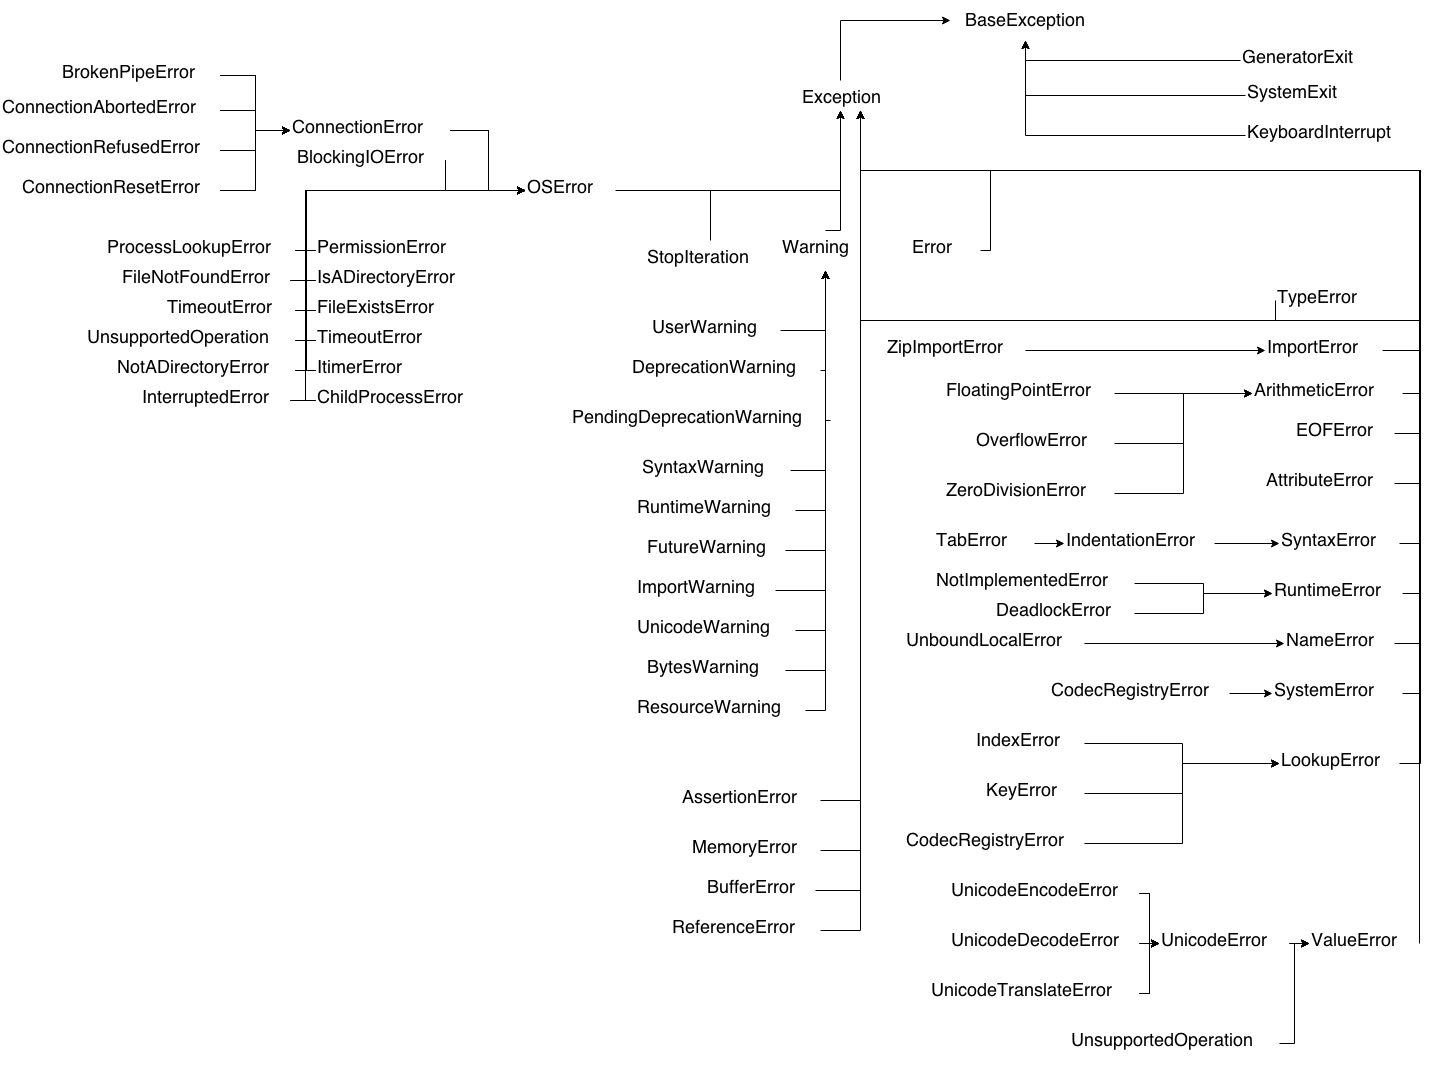
\includegraphics[height=0.8\textheight]{python_exceptions}
\end{frame}


\begin{frame}
  \frametitle{Catching exceptions}
  \begin{Verbatim}[label=\makebox{\url{https://github.com/lucabaldini/cmepda/tree/master/slides/latex/snippets/try\_block.py}},commandchars=\\\{\}]
\PY{k}{try}\PY{p}{:}
    \PY{k}{with} \PY{n+nb}{open} \PY{p}{(}\PY{l+s+s1}{\PYZsq{}}\PY{l+s+s1}{i\PYZus{}do\PYZus{}not\PYZus{}exist.txt}\PY{l+s+s1}{\PYZsq{}}\PY{p}{)} \PY{k}{as} \PY{n}{lab\PYZus{}data\PYZus{}file}\PY{p}{:}
        \PY{l+s+sd}{\PYZdq{}\PYZdq{}\PYZdq{} Do some process here...}
\PY{l+s+sd}{        \PYZdq{}\PYZdq{}\PYZdq{}}
        \PY{k}{pass}
        
\PY{k}{except} \PY{n}{FileNotFoundError} \PY{k}{as} \PY{n}{e}\PY{p}{:} \PY{c+c1}{\PYZsh{} we assign a name to the the exception }
    \PY{k}{print}\PY{p}{(}\PY{n}{e}\PY{p}{)}

\PY{c+c1}{\PYZsh{} We can be less specific by catching a parent exception}
\PY{k}{except} \PY{n+ne}{OSError} \PY{k}{as} \PY{n}{e}\PY{p}{:} \PY{c+c1}{\PYZsh{} OSError is a parent class of FileNotFoundError}
    \PY{k}{print}\PY{p}{(}\PY{n}{e}\PY{p}{)}

\PY{c+c1}{\PYZsh{} catching Exception will catch almost everything!}
\PY{k}{except} \PY{n+ne}{Exception} \PY{k}{as} \PY{n}{e}\PY{p}{:}
    \PY{k}{print}\PY{p}{(}\PY{n}{e}\PY{p}{)}

[Output]
[Errno 2] No such file or directory: 'i_do_not_exist.txt'
\end{Verbatim}
\end{frame}


\begin{frame}
  \frametitle{Raising exceptions}
  \begin{Verbatim}[label=\makebox{\url{https://github.com/lucabaldini/cmepda/tree/master/slides/latex/snippets/raising.py}},commandchars=\\\{\}]
\PY{k}{def} \PY{n+nf}{raising\PYZus{}function}\PY{p}{(}\PY{p}{)}\PY{p}{:}
    \PY{c+c1}{\PYZsh{} You can pass useful message to the exceptions you raise}
    \PY{k}{raise} \PY{n+ne}{RuntimeError}\PY{p}{(}\PY{l+s+s1}{\PYZsq{}}\PY{l+s+s1}{this is a useful debug message}\PY{l+s+s1}{\PYZsq{}}\PY{p}{)} 

\PY{k}{try}\PY{p}{:}
    \PY{n}{raising\PYZus{}function}\PY{p}{(}\PY{p}{)}
\PY{k}{except} \PY{n+ne}{RuntimeError} \PY{k}{as} \PY{n}{e}\PY{p}{:}
    \PY{c+c1}{\PYZsh{} The message can be retrieved by printing the exception}
    \PY{k}{print}\PY{p}{(}\PY{n}{e}\PY{p}{)}

[Output]
this is a useful debug message
\end{Verbatim}
\end{frame}


\begin{frame}
  \frametitle{Where to catch exceptions?}

  \begin{itemize}
    \item Differently from error flags, which needs to be checked as early as
          possible, you are not in a rush with exceptions
    \item Remeber: your goal is to provide the user a meaningful error message and
          useful debug information.
    \item You should catch an exception only when you have enough context to
          do that - which sometimes means waiting a few levels in the hierarchy!
  \end{itemize}
\end{frame}


\begin{frame}
  \frametitle{When to catch?}
  \centering
  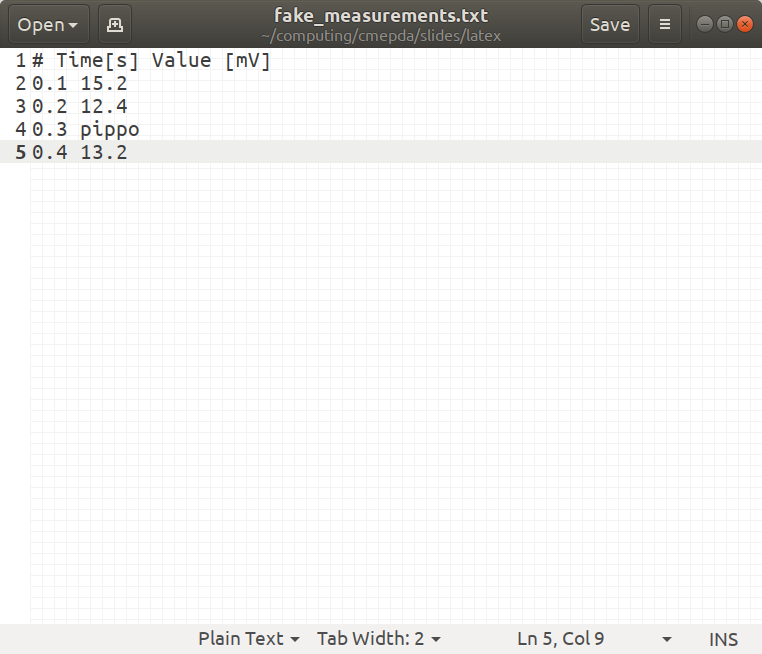
\includegraphics[width=0.8\textwidth]{lab_file.png}
\end{frame}



\begin{frame}
  \frametitle{When to catch?}
  \begin{Verbatim}[label=\makebox{\url{https://github.com/lucabaldini/cmepda/tree/master/slides/latex/snippets/when\_to\_catch.py}},commandchars=\\\{\}]
\PY{k}{def} \PY{n+nf}{parse\PYZus{}line}\PY{p}{(}\PY{n}{line}\PY{p}{)}\PY{p}{:}
    \PY{l+s+sd}{\PYZdq{}\PYZdq{}\PYZdq{} Parse a line of the file and return the values as float\PYZdq{}\PYZdq{}\PYZdq{}}
    \PY{n}{values} \PY{o}{=} \PY{n}{line}\PY{o}{.}\PY{n}{strip}\PY{p}{(}\PY{l+s+s1}{\PYZsq{}}\PY{l+s+se}{\PYZbs{}n}\PY{l+s+s1}{\PYZsq{}}\PY{p}{)}\PY{o}{.}\PY{n}{split}\PY{p}{(}\PY{l+s+s1}{\PYZsq{}}\PY{l+s+s1}{ }\PY{l+s+s1}{\PYZsq{}}\PY{p}{)}
    \PY{c+c1}{\PYZsh{} the following two lines may generate exceptions if they fails!}
    \PY{n}{time} \PY{o}{=} \PY{n+nb}{float}\PY{p}{(}\PY{n}{values}\PY{p}{[}\PY{l+m+mi}{0}\PY{p}{]}\PY{p}{)}
    \PY{n}{tension} \PY{o}{=} \PY{n+nb}{float}\PY{p}{(}\PY{n}{values}\PY{p}{[}\PY{l+m+mi}{1}\PY{p}{]}\PY{p}{)}
    \PY{k}{return} \PY{n}{time}\PY{p}{,} \PY{n}{tension}

\PY{k}{with} \PY{n+nb}{open}\PY{p}{(}\PY{l+s+s1}{\PYZsq{}}\PY{l+s+s1}{snippets/data/fake\PYZus{}measurements.txt}\PY{l+s+s1}{\PYZsq{}}\PY{p}{)} \PY{k}{as} \PY{n}{lab\PYZus{}data\PYZus{}file}\PY{p}{:}
    \PY{k}{for} \PY{n}{line} \PY{o+ow}{in} \PY{n}{lab\PYZus{}data\PYZus{}file}\PY{p}{:}
        \PY{k}{if} \PY{o+ow}{not} \PY{n}{line}\PY{o}{.}\PY{n}{startswith}\PY{p}{(}\PY{l+s+s1}{\PYZsq{}}\PY{l+s+s1}{\PYZsh{}}\PY{l+s+s1}{\PYZsq{}}\PY{p}{)}\PY{p}{:} \PY{c+c1}{\PYZsh{} skip comments}
            \PY{n}{time}\PY{p}{,} \PY{n}{tension} \PY{o}{=} \PY{n}{parse\PYZus{}line}\PY{p}{(}\PY{n}{line}\PY{p}{)}
            \PY{k}{print}\PY{p}{(}\PY{n}{time}\PY{p}{,} \PY{n}{tension}\PY{p}{)}

[Output]
0.1 15.2
0.2 12.4
Traceback (most recent call last):
  File "snippets/when_to_catch.py", line 12, in <module>
    time, tension = parse_line(line)
  File "snippets/when_to_catch.py", line 6, in parse_line
    tension = float(values[1])
ValueError: could not convert string to float: 'pippo'
\end{Verbatim}
\end{frame}


\begin{frame}
  \frametitle{Catch too early}
  \begin{Verbatim}[label=\makebox{\url{https://github.com/lucabaldini/cmepda/tree/master/slides/latex/snippets/when\_to\_catch\_1.py}},commandchars=\\\{\}]
\PY{k}{def} \PY{n+nf}{parse\PYZus{}line}\PY{p}{(}\PY{n}{line}\PY{p}{)}\PY{p}{:}
    \PY{l+s+sd}{\PYZdq{}\PYZdq{}\PYZdq{} Parse a line of the file and return the values as float\PYZdq{}\PYZdq{}\PYZdq{}}
    \PY{n}{values} \PY{o}{=} \PY{n}{line}\PY{o}{.}\PY{n}{strip}\PY{p}{(}\PY{l+s+s1}{\PYZsq{}}\PY{l+s+se}{\PYZbs{}n}\PY{l+s+s1}{\PYZsq{}}\PY{p}{)}\PY{o}{.}\PY{n}{split}\PY{p}{(}\PY{l+s+s1}{\PYZsq{}}\PY{l+s+s1}{ }\PY{l+s+s1}{\PYZsq{}}\PY{p}{)}
    \PY{k}{try}\PY{p}{:}
        \PY{n}{time} \PY{o}{=} \PY{n+nb}{float}\PY{p}{(}\PY{n}{values}\PY{p}{[}\PY{l+m+mi}{0}\PY{p}{]}\PY{p}{)}
        \PY{n}{tension} \PY{o}{=} \PY{n+nb}{float}\PY{p}{(}\PY{n}{values}\PY{p}{[}\PY{l+m+mi}{1}\PY{p}{]}\PY{p}{)}
    \PY{k}{except} \PY{n+ne}{ValueError} \PY{k}{as} \PY{n}{e}\PY{p}{:}
        \PY{k}{print}\PY{p}{(}\PY{n}{e}\PY{p}{)} \PY{c+c1}{\PYZsh{} This is not useful \PYZhy{} which line of the file has the error?}
        \PY{k}{return} \PY{n+nb+bp}{None} \PY{c+c1}{\PYZsh{} We can\PYZsq{}t really return something meaningful}
    \PY{k}{return} \PY{n}{time}\PY{p}{,} \PY{n}{tension}

\PY{k}{with} \PY{n+nb}{open}\PY{p}{(}\PY{l+s+s1}{\PYZsq{}}\PY{l+s+s1}{measurements.txt}\PY{l+s+s1}{\PYZsq{}}\PY{p}{)} \PY{k}{as} \PY{n}{lab\PYZus{}data\PYZus{}file}\PY{p}{:}
    \PY{k}{for} \PY{n}{line} \PY{o+ow}{in} \PY{n}{lab\PYZus{}data\PYZus{}file}\PY{p}{:}
        \PY{k}{if} \PY{o+ow}{not} \PY{n}{line}\PY{o}{.}\PY{n}{startswith}\PY{p}{(}\PY{l+s+s1}{\PYZsq{}}\PY{l+s+s1}{\PYZsh{}}\PY{l+s+s1}{\PYZsq{}}\PY{p}{)}\PY{p}{:} \PY{c+c1}{\PYZsh{} skip comments}
            \PY{n}{time}\PY{p}{,} \PY{n}{tension} \PY{o}{=} \PY{n}{parse\PYZus{}line}\PY{p}{(}\PY{n}{line}\PY{p}{)}
            \PY{k}{print}\PY{p}{(}\PY{n}{time}\PY{p}{,} \PY{n}{tension}\PY{p}{)} \PY{c+c1}{\PYZsh{} This line still crash badly!}

[Output]
0.1 15.2
0.2 12.4
could not convert string to float: 'pippo'
Traceback (most recent call last):
  File "snippets/when_to_catch_1.py", line 15, in <module>
    time, tension = parse_line(line)
TypeError: 'NoneType' object is not iterable
\end{Verbatim}
\end{frame}


\begin{frame}
  \frametitle{Catch when needed}
  \begin{Verbatim}[label=\makebox{\url{https://github.com/lucabaldini/cmepda/tree/master/slides/latex/snippets/when\_to\_catch\_2.py}},commandchars=\\\{\}]
\PY{k}{def} \PY{n+nf}{parse\PYZus{}line}\PY{p}{(}\PY{n}{line}\PY{p}{)}\PY{p}{:}
    \PY{l+s+sd}{\PYZdq{}\PYZdq{}\PYZdq{} Parse a line of the file and return the values as float\PYZdq{}\PYZdq{}\PYZdq{}}
    \PY{n}{values} \PY{o}{=} \PY{n}{line}\PY{o}{.}\PY{n}{strip}\PY{p}{(}\PY{l+s+s1}{\PYZsq{}}\PY{l+s+se}{\PYZbs{}n}\PY{l+s+s1}{\PYZsq{}}\PY{p}{)}\PY{o}{.}\PY{n}{split}\PY{p}{(}\PY{l+s+s1}{\PYZsq{}}\PY{l+s+s1}{ }\PY{l+s+s1}{\PYZsq{}}\PY{p}{)}
    \PY{c+c1}{\PYZsh{} the following two lines may generate exceptions if they fails!}
    \PY{n}{time} \PY{o}{=} \PY{n+nb}{float}\PY{p}{(}\PY{n}{values}\PY{p}{[}\PY{l+m+mi}{0}\PY{p}{]}\PY{p}{)}
    \PY{n}{tension} \PY{o}{=} \PY{n+nb}{float}\PY{p}{(}\PY{n}{values}\PY{p}{[}\PY{l+m+mi}{1}\PY{p}{]}\PY{p}{)}
    \PY{k}{return} \PY{n}{time}\PY{p}{,} \PY{n}{tension}

\PY{k}{with} \PY{n+nb}{open}\PY{p}{(}\PY{l+s+s1}{\PYZsq{}}\PY{l+s+s1}{measurements.txt}\PY{l+s+s1}{\PYZsq{}}\PY{p}{)} \PY{k}{as} \PY{n}{lab\PYZus{}data\PYZus{}file}\PY{p}{:}
    \PY{k}{for} \PY{n}{line\PYZus{}number}\PY{p}{,} \PY{n}{line} \PY{o+ow}{in} \PY{n+nb}{enumerate}\PY{p}{(}\PY{n}{lab\PYZus{}data\PYZus{}file}\PY{p}{)}\PY{p}{:} \PY{c+c1}{\PYZsh{} get the line number}
        \PY{k}{if} \PY{o+ow}{not} \PY{n}{line}\PY{o}{.}\PY{n}{startswith}\PY{p}{(}\PY{l+s+s1}{\PYZsq{}}\PY{l+s+s1}{\PYZsh{}}\PY{l+s+s1}{\PYZsq{}}\PY{p}{)}\PY{p}{:} \PY{c+c1}{\PYZsh{} skip comments}
            \PY{k}{try}\PY{p}{:}
                \PY{n}{time}\PY{p}{,} \PY{n}{tension} \PY{o}{=} \PY{n}{parse\PYZus{}line}\PY{p}{(}\PY{n}{line}\PY{p}{)}
                \PY{k}{print}\PY{p}{(}\PY{n}{time}\PY{p}{,} \PY{n}{tension}\PY{p}{)}
            \PY{k}{except} \PY{n+ne}{ValueError} \PY{k}{as} \PY{n}{e}\PY{p}{:}
                \PY{k}{print}\PY{p}{(}\PY{l+s+s1}{\PYZsq{}}\PY{l+s+s1}{Line \PYZob{}\PYZcb{} error: \PYZob{}\PYZcb{}}\PY{l+s+s1}{\PYZsq{}}\PY{o}{.}\PY{n}{format}\PY{p}{(}\PY{n}{line\PYZus{}number}\PY{p}{,} \PY{n}{e}\PY{p}{)}\PY{p}{)}

[Output]
0.1 15.2
0.2 12.4
Line 3 error: could not convert string to float: 'pippo'
0.4 13.2
\end{Verbatim}
\end{frame}

\begin{frame}
  \frametitle{There is no check - only try}

  \begin{itemize}
    \item In Python exceptions are the default methods for handling failures
    \item Many functions raise an exception when something goes wrong
    \item The common approach is: do not chech the input beforehand. Use it and
          be ready to catch excpetions if any.
    \item \textit{Easier to ask for forgiveness than permission.} 
  \end{itemize}
\end{frame}


\begin{frame}
  \frametitle{Easier to ask for forgiveness}
  \begin{Verbatim}[label=\makebox{\url{https://github.com/lucabaldini/cmepda/tree/master/slides/latex/snippets/dont\_ask\_permission.py}},commandchars=\\\{\}]
\PY{k+kn}{import} \PY{n+nn}{os}

\PY{n}{file\PYZus{}path} \PY{o}{=} \PY{l+s+s1}{\PYZsq{}}\PY{l+s+s1}{i\PYZus{}do\PYZus{}not\PYZus{}exists.txt}\PY{l+s+s1}{\PYZsq{}}

\PY{c+c1}{\PYZsh{} Defensive version}
\PY{k}{if} \PY{n}{os}\PY{o}{.}\PY{n}{path}\PY{o}{.}\PY{n}{exists}\PY{p}{(}\PY{n}{file\PYZus{}path}\PY{p}{)}\PY{p}{:}
    \PY{c+c1}{\PYZsh{} What if the file is deleted between these two lines? (by another process)}
    \PY{c+c1}{\PYZsh{} What if the file exists but you don\PYZsq{}t have permission to open it?}
    \PY{n}{data\PYZus{}file} \PY{o}{=} \PY{n+nb}{open}\PY{p}{(}\PY{n}{file\PYZus{}path}\PY{p}{)} 
\PY{k}{else}\PY{p}{:}
    \PY{c+c1}{\PYZsh{} Do something}
    \PY{k}{print}\PY{p}{(}\PY{l+s+s1}{\PYZsq{}}\PY{l+s+s1}{Oops \PYZhy{} file }\PY{l+s+se}{\PYZbs{}\PYZsq{}}\PY{l+s+s1}{\PYZob{}\PYZcb{}}\PY{l+s+se}{\PYZbs{}\PYZsq{}}\PY{l+s+s1}{ does not exist}\PY{l+s+s1}{\PYZsq{}}\PY{o}{.}\PY{n}{format}\PY{p}{(}\PY{n}{file\PYZus{}path}\PY{p}{)}\PY{p}{)}

\PY{c+c1}{\PYZsh{} Pythonic way \PYZhy{} you should prefer this one!}
\PY{k}{try}\PY{p}{:}
    \PY{n}{data\PYZus{}file} \PY{o}{=} \PY{n+nb}{open}\PY{p}{(}\PY{n}{file\PYZus{}path}\PY{p}{)}
\PY{k}{except} \PY{n+ne}{OSError} \PY{k}{as} \PY{n}{e}\PY{p}{:} \PY{c+c1}{\PYZsh{} Cover more problems than FileNotFoundError}
    \PY{k}{print}\PY{p}{(}\PY{l+s+s1}{\PYZsq{}}\PY{l+s+s1}{Oops \PYZhy{} cannot read the file!}\PY{l+s+se}{\PYZbs{}n}\PY{l+s+s1}{\PYZob{}\PYZcb{}}\PY{l+s+s1}{\PYZsq{}}\PY{o}{.}\PY{n}{format}\PY{p}{(}\PY{n}{e}\PY{p}{)}\PY{p}{)}

[Output]
Oops - file 'i_do_not_exists.txt' does not exist
Oops - cannot read the file!
[Errno 2] No such file or directory: 'i_do_not_exists.txt'
\end{Verbatim}
\end{frame}


\begin{frame}
  \frametitle{}
    \centering \Large Decorators
\end{frame}


\begin{frame}
  \frametitle{Functions inside functions}
  \begin{itemize}
    \item Function in python are \alert{first class object}
    \item The name is a bit misleading, but what actually means is that functions
          can be passed as argument to other functions and returned as result from
          other functions
    \item This shouldn't surprise you much: functions are objects of a
          '\emph{function}' class, so they behave like any other vairable in
          Python
    \item Another thing you can (and sometimes want to) do is \emph{defining} a
          function inside another.
    \item Let's see how it works
  \end{itemize}
  
\end{frame}


\begin{frame}
  \frametitle{Functions inside functions}
  \begin{Verbatim}[label=\makebox{\url{https://github.com/lucabaldini/cmepda/tree/master/slides/latex/snippets/inner\_outer.py}},commandchars=\\\{\}]
\PY{k}{def} \PY{n+nf}{outer}\PY{p}{(}\PY{p}{)}\PY{p}{:}   
    \PY{k}{def} \PY{n+nf}{inner}\PY{p}{(}\PY{p}{)}\PY{p}{:} \PY{c+c1}{\PYZsh{} Defining the inner function inside the outer function}
        \PY{k}{print}\PY{p}{(}\PY{l+s+s1}{\PYZsq{}}\PY{l+s+s1}{Inner function}\PY{l+s+s1}{\PYZsq{}}\PY{p}{)}
        \PY{k}{return} \PY{c+c1}{\PYZsh{} End of the inner function}
    \PY{k}{return} \PY{n}{inner} \PY{c+c1}{\PYZsh{} Inner is the output of outer}
    
\PY{n}{my\PYZus{}func} \PY{o}{=} \PY{n}{outer}\PY{p}{(}\PY{p}{)} \PY{c+c1}{\PYZsh{} my\PYZus{}func is now referncing \PYZsq{}inner\PYZsq{}}
\PY{k}{print}\PY{p}{(}\PY{n}{my\PYZus{}func}\PY{o}{.}\PY{n+nv+vm}{\PYZus{}\PYZus{}name\PYZus{}\PYZus{}}\PY{p}{)}
\PY{n}{my\PYZus{}func}\PY{p}{(}\PY{p}{)} \PY{c+c1}{\PYZsh{} Calling my\PYZus{}func is equal to calling \PYZsq{}inner\PYZsq{}}

\PY{k}{def} \PY{n+nf}{outer2}\PY{p}{(}\PY{p}{)}\PY{p}{:}
    \PY{n}{some\PYZus{}string} \PY{o}{=} \PY{l+s+s1}{\PYZsq{}}\PY{l+s+s1}{Hello!}\PY{l+s+s1}{\PYZsq{}}
    \PY{k}{def} \PY{n+nf}{inner}\PY{p}{(}\PY{p}{)}\PY{p}{:}
        \PY{c+c1}{\PYZsh{} We have access to the variables in the outer function!}
        \PY{k}{print}\PY{p}{(}\PY{n}{some\PYZus{}string}\PY{p}{)}
    \PY{k}{return} \PY{n}{inner}
    
\PY{n}{my\PYZus{}other\PYZus{}func} \PY{o}{=} \PY{n}{outer2}\PY{p}{(}\PY{p}{)}
\PY{n}{my\PYZus{}other\PYZus{}func}\PY{p}{(}\PY{p}{)}

[Output]
inner
Inner function
Hello!
\end{Verbatim}
\end{frame}


\begin{frame}
  \frametitle{Colsures and free variables}
  \begin{itemize}
    \item When a function is created inside another function it has access to the local variables
          of the outer function, even after its scope ended
    \item This is techincally possible because those varibales are kept in a special
          space of memory, the \alert{closure} of the inner function
    \item Such variables are called \alert{free variables}
    \item Note: if you \emph{assign} to a free variable in the inner function, 
          by default a new, local variable is created instead!
    \item To avoid this you have to explictly declare that you want to access the variable in
          the closure using the \alert{nonlocal} keyword
    \item Remember: \emph{'Explicit is better then implicit'}
  \end{itemize}
  
\end{frame}


\begin{frame}
  \frametitle{Free variables - a mistake to avoid}
  \begin{Verbatim}[label=\makebox{\url{https://github.com/lucabaldini/cmepda/tree/master/slides/latex/snippets/closure\_wrong.py}},commandchars=\\\{\}]
\PY{k}{def} \PY{n+nf}{running\PYZus{}average}\PY{p}{(}\PY{p}{)}\PY{p}{:}
    \PY{n}{total\PYZus{}count} \PY{o}{=} \PY{l+m+mi}{0}
    \PY{n}{num\PYZus{}elements} \PY{o}{=} \PY{l+m+mi}{0}
    \PY{k}{def} \PY{n+nf}{accumulator}\PY{p}{(}\PY{n}{value}\PY{p}{)}\PY{p}{:}
        \PY{n}{total\PYZus{}count} \PY{o}{+}\PY{o}{=} \PY{n}{value} \PY{c+c1}{\PYZsh{} Doesn\PYZsq{}t work! total\PYZus{}count is reassigned!}
        \PY{n}{num\PYZus{}elements} \PY{o}{+}\PY{o}{=} \PY{l+m+mi}{1} \PY{c+c1}{\PYZsh{} Doesn\PYZsq{}t work! total\PYZus{}count is reassigned!}
        \PY{k}{return} \PY{n}{total\PYZus{}count}\PY{o}{/}\PY{n}{num\PYZus{}elements}
    \PY{k}{return} \PY{n}{accumulator}
    
\PY{n}{run\PYZus{}avg} \PY{o}{=} \PY{n}{running\PYZus{}average}\PY{p}{(}\PY{p}{)}
\PY{k}{print}\PY{p}{(}\PY{n}{run\PYZus{}avg}\PY{p}{(}\PY{l+m+mf}{1.}\PY{p}{)}\PY{p}{)}
\PY{k}{print}\PY{p}{(}\PY{n}{run\PYZus{}avg}\PY{p}{(}\PY{l+m+mf}{5.}\PY{p}{)}\PY{p}{)}
\PY{k}{print}\PY{p}{(}\PY{n}{run\PYZus{}avg}\PY{p}{(}\PY{l+m+mf}{2.5}\PY{p}{)}\PY{p}{)}

[Output]
Traceback (most recent call last):
  File "snippets/closure_wrong.py", line 11, in <module>
    print(run_avg(1.))
  File "snippets/closure_wrong.py", line 5, in accumulator
    total_count += value # Doesn't work! total_count is reassigned!
UnboundLocalError: local variable 'total_count' referenced before assignment
\end{Verbatim}
\end{frame}


\begin{frame}
  \frametitle{Free variables - the correct way}
  \begin{Verbatim}[label=\makebox{\url{https://github.com/lucabaldini/cmepda/tree/master/slides/latex/snippets/closure\_right.py}},commandchars=\\\{\}]
\PY{k}{def} \PY{n+nf}{running\PYZus{}average}\PY{p}{(}\PY{p}{)}\PY{p}{:}
    \PY{n}{total\PYZus{}count} \PY{o}{=} \PY{l+m+mi}{0}
    \PY{n}{num\PYZus{}elements} \PY{o}{=} \PY{l+m+mi}{0}
    \PY{k}{def} \PY{n+nf}{accumulator}\PY{p}{(}\PY{n}{value}\PY{p}{)}\PY{p}{:}
        \PY{c+c1}{\PYZsh{} We declare the relevant variables as nonlocal}
        \PY{n}{nonlocal} \PY{n}{total\PYZus{}count}\PY{p}{,} \PY{n}{num\PYZus{}elements}
        \PY{c+c1}{\PYZsh{} Now we can assign to them \PYZhy{} the variables in the closure will be}
        \PY{c+c1}{\PYZsh{} modified, as we want!}
        \PY{n}{total\PYZus{}count} \PY{o}{+}\PY{o}{=} \PY{n}{value}
        \PY{n}{num\PYZus{}elements} \PY{o}{+}\PY{o}{=} \PY{l+m+mi}{1}
        \PY{k}{return} \PY{n}{total\PYZus{}count}\PY{o}{/}\PY{n}{num\PYZus{}elements}
    \PY{k}{return} \PY{n}{accumulator}
    
\PY{n}{run\PYZus{}avg} \PY{o}{=} \PY{n}{running\PYZus{}average}\PY{p}{(}\PY{p}{)}
\PY{k}{print}\PY{p}{(}\PY{n}{run\PYZus{}avg}\PY{p}{(}\PY{l+m+mf}{1.}\PY{p}{)}\PY{p}{)}
\PY{k}{print}\PY{p}{(}\PY{n}{run\PYZus{}avg}\PY{p}{(}\PY{l+m+mf}{5.}\PY{p}{)}\PY{p}{)}
\PY{k}{print}\PY{p}{(}\PY{n}{run\PYZus{}avg}\PY{p}{(}\PY{l+m+mf}{2.5}\PY{p}{)}\PY{p}{)}

[Output]
1.0
3.0
2.8333333333333335
\end{Verbatim}
\end{frame}


\begin{frame}
  \frametitle{Wrapping functions}
  \begin{itemize}
    \item The typical use of defining a function inside a function is to create
          a \alert{wrapper}
    \item A wrapper is a function that calls another one adding a layer
          of functionalities in between - for example it may do some pre-process
          of the input, or change the output in some way, or measure the 
          execution time or whatever we want
    \item The techinque for creating a wrapper fucntion in Python is:
    \begin{itemize}
       \item Pass the function that we want to wrap as argument of the outer
             function
       \item Inside the outer function we define an inner function, which is the
             actual wrapper
       \item The wrapper calls the wrapped function and adds its functionalities,
             before and/or after the call. It may return the same output or a 
             manipulated one.
       \item Then from the outer fucntion we return the wrapper
    \end{itemize}
  \end{itemize}
  
\end{frame}


\begin{frame}
  \frametitle{Wrapper}
  \begin{Verbatim}[label=\makebox{\url{https://github.com/lucabaldini/cmepda/tree/master/slides/latex/snippets/wrapper.py}},commandchars=\\\{\}]
\PY{k}{def} \PY{n+nf}{some\PYZus{}function}\PY{p}{(}\PY{n}{a}\PY{p}{,} \PY{n}{b}\PY{p}{)}\PY{p}{:}
    \PY{k}{print}\PY{p}{(}\PY{l+s+s1}{\PYZsq{}}\PY{l+s+s1}{Executing \PYZob{}\PYZcb{} x \PYZob{}\PYZcb{}}\PY{l+s+s1}{\PYZsq{}}\PY{o}{.}\PY{n}{format}\PY{p}{(}\PY{n}{a}\PY{p}{,} \PY{n}{b}\PY{p}{)}\PY{p}{)}
    \PY{k}{return} \PY{n}{a} \PY{o}{*} \PY{n}{b}
    
\PY{k}{def} \PY{n+nf}{add\PYZus{}n\PYZus{}wrapper}\PY{p}{(}\PY{n}{func}\PY{p}{,} \PY{n}{n}\PY{p}{)}\PY{p}{:} \PY{c+c1}{\PYZsh{} We take the wrapped function as argument}
    \PY{l+s+sd}{\PYZdq{}\PYZdq{}\PYZdq{} This wrapper adds n to the result of the wrapped function\PYZdq{}\PYZdq{}\PYZdq{}}
    
    \PY{k}{def} \PY{n+nf}{wrapper}\PY{p}{(}\PY{o}{*}\PY{n}{args}\PY{p}{,} \PY{o}{*}\PY{o}{*}\PY{n}{kwargs}\PY{p}{)}\PY{p}{:} 
       \PY{l+s+sd}{\PYZdq{}\PYZdq{}\PYZdq{}We passs the arguments as *arg, **kwargs, because this is the most}
\PY{l+s+sd}{       general form in Python: we can collect any comination of arguments like}
\PY{l+s+sd}{       that. Note that we have access to both \PYZsq{}func\PYZsq{} and \PYZsq{}n\PYZsq{}, as they are stored}
\PY{l+s+sd}{       in the closure of \PYZsq{}wrapper\PYZsq{}\PYZdq{}\PYZdq{}\PYZdq{}}
       \PY{n}{result} \PY{o}{=} \PY{n}{func}\PY{p}{(}\PY{o}{*}\PY{n}{args}\PY{p}{,} \PY{o}{*}\PY{o}{*}\PY{n}{kwargs}\PY{p}{)} \PY{c+c1}{\PYZsh{} Pass the arguments to the wrapped fucntion}
       \PY{k}{print}\PY{p}{(}\PY{l+s+s1}{\PYZsq{}}\PY{l+s+s1}{Adding \PYZob{}\PYZcb{}}\PY{l+s+s1}{\PYZsq{}}\PY{o}{.}\PY{n}{format}\PY{p}{(}\PY{n}{n}\PY{p}{)}\PY{p}{)}
       \PY{k}{return} \PY{n}{result} \PY{o}{+} \PY{n}{n} \PY{c+c1}{\PYZsh{} Return a modified result in this case}
       
    \PY{k}{return} \PY{n}{wrapper} \PY{c+c1}{\PYZsh{} From add\PYZus{}n\PYZus{}wrapper we return the wrapper}

\PY{n}{function\PYZus{}plus\PYZus{}five} \PY{o}{=} \PY{n}{add\PYZus{}n\PYZus{}wrapper}\PY{p}{(}\PY{n}{some\PYZus{}function}\PY{p}{,} \PY{l+m+mi}{5}\PY{p}{)}
\PY{k}{print}\PY{p}{(}\PY{l+s+s1}{\PYZsq{}}\PY{l+s+s1}{Result = \PYZob{}\PYZcb{}}\PY{l+s+s1}{\PYZsq{}}\PY{o}{.}\PY{n}{format}\PY{p}{(}\PY{n}{function\PYZus{}plus\PYZus{}five}\PY{p}{(}\PY{l+m+mi}{2}\PY{p}{,} \PY{l+m+mi}{3}\PY{p}{)}\PY{p}{)}\PY{p}{)}

[Output]
Executing 2 x 3
Adding 5
Result = 11
\end{Verbatim}
\end{frame}


\begin{frame}
  \frametitle{Decorators}
  \begin{itemize}
    \item Often, when you wrap a function, you don't want to change
          it's name, so you reassign the wrapped funtion to its old name
    \item In fact, this techinque is so common that python introduced a special
          syntax for it: decorators
    \item A decorated function has simply the name of the wrapper added with
          a '@' on top of its declaration
  \end{itemize}
  
\end{frame}


\begin{frame}
  \frametitle{Decorators}
  \begin{Verbatim}[label=\makebox{\url{https://github.com/lucabaldini/cmepda/tree/master/slides/latex/snippets/decorator.py}},commandchars=\\\{\}]
\PY{k}{def} \PY{n+nf}{print\PYZus{}function\PYZus{}info}\PY{p}{(}\PY{n}{func}\PY{p}{)}\PY{p}{:}
    \PY{k}{def} \PY{n+nf}{wrapper}\PY{p}{(}\PY{o}{*}\PY{n}{args}\PY{p}{,} \PY{o}{*}\PY{o}{*}\PY{n}{kwargs}\PY{p}{)}\PY{p}{:}
        \PY{k}{print}\PY{p}{(}\PY{l+s+s1}{\PYZsq{}}\PY{l+s+s1}{Calling function }\PY{l+s+se}{\PYZbs{}\PYZsq{}}\PY{l+s+s1}{\PYZob{}\PYZcb{}}\PY{l+s+se}{\PYZbs{}\PYZsq{}}\PY{l+s+s1}{\PYZsq{}}\PY{o}{.}\PY{n}{format}\PY{p}{(}\PY{n}{func}\PY{o}{.}\PY{n+nv+vm}{\PYZus{}\PYZus{}name\PYZus{}\PYZus{}}\PY{p}{)}\PY{p}{)}
        \PY{k}{print}\PY{p}{(}\PY{l+s+s1}{\PYZsq{}}\PY{l+s+s1}{Positional arguments = \PYZob{}\PYZcb{}}\PY{l+s+s1}{\PYZsq{}}\PY{o}{.}\PY{n}{format}\PY{p}{(}\PY{n}{args}\PY{p}{)}\PY{p}{)}
        \PY{k}{print}\PY{p}{(}\PY{l+s+s1}{\PYZsq{}}\PY{l+s+s1}{Keyword arguments = \PYZob{}\PYZcb{}}\PY{l+s+s1}{\PYZsq{}}\PY{o}{.}\PY{n}{format}\PY{p}{(}\PY{n}{kwargs}\PY{p}{)}\PY{p}{)}
        \PY{k}{return} \PY{n}{func}\PY{p}{(}\PY{o}{*}\PY{n}{args}\PY{p}{,} \PY{o}{*}\PY{o}{*}\PY{n}{kwargs}\PY{p}{)}
    \PY{k}{return} \PY{n}{wrapper}

\PY{n+nd}{@print\PYZus{}function\PYZus{}info}
\PY{k}{def} \PY{n+nf}{some\PYZus{}function}\PY{p}{(}\PY{n}{a}\PY{p}{,} \PY{n}{b}\PY{p}{,} \PY{n}{c}\PY{o}{=}\PY{l+m+mi}{0}\PY{p}{)}\PY{p}{:}
    \PY{k}{return} \PY{n}{a} \PY{o}{*} \PY{n}{b} \PY{o}{+} \PY{n}{c}

\PY{c+c1}{\PYZsh{} This is equivalent to: some\PYZus{}function = print\PYZus{}function\PYZus{}info(some\PYZus{}function)}

\PY{k}{print}\PY{p}{(}\PY{n}{some\PYZus{}function}\PY{p}{(}\PY{l+m+mi}{1}\PY{p}{,} \PY{l+m+mi}{2}\PY{p}{,} \PY{n}{c}\PY{o}{=}\PY{l+m+mi}{7}\PY{p}{)}\PY{p}{)}
 \PY{c+c1}{\PYZsh{} Inspecting the function reveals that we are calling the wrapper}
\PY{k}{print}\PY{p}{(}\PY{l+s+s1}{\PYZsq{}}\PY{l+s+s1}{The name of the function is }\PY{l+s+se}{\PYZbs{}\PYZsq{}}\PY{l+s+s1}{\PYZob{}\PYZcb{}}\PY{l+s+se}{\PYZbs{}\PYZsq{}}\PY{l+s+s1}{\PYZsq{}}\PY{o}{.}\PY{n}{format}\PY{p}{(}\PY{n}{some\PYZus{}function}\PY{o}{.}\PY{n+nv+vm}{\PYZus{}\PYZus{}name\PYZus{}\PYZus{}}\PY{p}{)}\PY{p}{)}

[Output]
Calling function 'some_function'
Positional arguments = (1, 2)
Keyword arguments = {'c': 7}
9
The name of the function is 'wrapper'
\end{Verbatim}
\end{frame}


\begin{frame}
  \frametitle{A decorator to measure execution time}
  \begin{Verbatim}[label=\makebox{\url{https://github.com/lucabaldini/cmepda/tree/master/slides/latex/snippets/time\_measuring\_decor.py}},commandchars=\\\{\}]
\PY{k+kn}{import} \PY{n+nn}{time} 
\PY{k+kn}{from} \PY{n+nn}{functools} \PY{k+kn}{import} \PY{n}{wraps}

\PY{k}{def} \PY{n+nf}{clocked}\PY{p}{(}\PY{n}{func}\PY{p}{)}\PY{p}{:}
    \PY{l+s+sd}{\PYZdq{}\PYZdq{}\PYZdq{} We use functools.wraps to keep the original function name and docstring\PYZdq{}\PYZdq{}\PYZdq{}}
    \PY{n+nd}{@wraps}\PY{p}{(}\PY{n}{func}\PY{p}{)}
    \PY{k}{def} \PY{n+nf}{wrapper}\PY{p}{(}\PY{o}{*}\PY{n}{args}\PY{p}{,} \PY{o}{*}\PY{o}{*}\PY{n}{kwargs}\PY{p}{)}\PY{p}{:}
        \PY{n}{tstart} \PY{o}{=} \PY{n}{time}\PY{o}{.}\PY{n}{clock}\PY{p}{(}\PY{p}{)}
        \PY{n}{result} \PY{o}{=} \PY{n}{func}\PY{p}{(}\PY{o}{*}\PY{n}{args}\PY{p}{,} \PY{o}{*}\PY{o}{*}\PY{n}{kwargs}\PY{p}{)}
        \PY{n}{exec\PYZus{}time} \PY{o}{=} \PY{n}{time}\PY{o}{.}\PY{n}{clock}\PY{p}{(}\PY{p}{)} \PY{o}{\PYZhy{}} \PY{n}{tstart}
        \PY{k}{print}\PY{p}{(}\PY{l+s+s1}{\PYZsq{}}\PY{l+s+s1}{Function \PYZob{}\PYZcb{} executed in \PYZob{}\PYZcb{} s}\PY{l+s+s1}{\PYZsq{}}\PY{o}{.}\PY{n}{format}\PY{p}{(}\PY{n}{func}\PY{o}{.}\PY{n+nv+vm}{\PYZus{}\PYZus{}name\PYZus{}\PYZus{}}\PY{p}{,} \PY{n}{exec\PYZus{}time}\PY{p}{)}\PY{p}{)}
        \PY{k}{return} \PY{n}{result}
    \PY{k}{return} \PY{n}{wrapper}

\PY{n+nd}{@clocked}
\PY{k}{def} \PY{n+nf}{square\PYZus{}list}\PY{p}{(}\PY{n}{input\PYZus{}list}\PY{p}{)}\PY{p}{:}
    \PY{l+s+sd}{\PYZdq{}\PYZdq{}\PYZdq{} Return the square of a list\PYZdq{}\PYZdq{}\PYZdq{}}
    \PY{k}{return} \PY{p}{[}\PY{n}{item}\PY{o}{*}\PY{o}{*}\PY{l+m+mi}{2} \PY{k}{for} \PY{n}{item} \PY{o+ow}{in} \PY{n}{input\PYZus{}list}\PY{p}{]}

\PY{c+c1}{\PYZsh{} Make sure the function name and docstring look the same}
\PY{k}{print}\PY{p}{(}\PY{l+s+s1}{\PYZsq{}}\PY{l+s+se}{\PYZbs{}\PYZsq{}}\PY{l+s+s1}{\PYZob{}\PYZcb{}}\PY{l+s+se}{\PYZbs{}\PYZsq{}}\PY{l+s+s1}{: \PYZob{}\PYZcb{}}\PY{l+s+s1}{\PYZsq{}}\PY{o}{.}\PY{n}{format}\PY{p}{(}\PY{n}{square\PYZus{}list}\PY{o}{.}\PY{n+nv+vm}{\PYZus{}\PYZus{}name\PYZus{}\PYZus{}}\PY{p}{,} \PY{n}{square\PYZus{}list}\PY{o}{.}\PY{n+nv+vm}{\PYZus{}\PYZus{}doc\PYZus{}\PYZus{}}\PY{p}{)}\PY{p}{)}
\PY{n}{square\PYZus{}list}\PY{p}{(}\PY{n+nb}{range}\PY{p}{(}\PY{l+m+mi}{2000000}\PY{p}{)}\PY{p}{)}

[Output]
'square_list':  Return the square of a list
Function square_list executed in 0.372302 s
\end{Verbatim}
\end{frame}


\begin{frame}
  \frametitle{The @classmethod decorator}
  \begin{itemize}
    \item We have already seen a built-in Python decorator: \emph{@property}
    \item We used that to get proper encapsulation
    \item There is another built-in decorator one which is very useful for classes: \alert{\emph{@classmethod}}
    \item A classmethod is like a class attribute: you don't need an instance to
          use it
    \item A class method can access class attributes but not instance attributes
    \item The main use for class methods is to provide \alert{alternate constructors}
  \end{itemize}
  
\end{frame}


\begin{frame}
  \frametitle{Class method}
  \begin{Verbatim}[label=\makebox{\url{https://github.com/lucabaldini/cmepda/tree/master/slides/latex/snippets/classmethod.py}},commandchars=\\\{\}]
\PY{k+kn}{import} \PY{n+nn}{numpy}

\PY{k}{class} \PY{n+nc}{LabData}\PY{p}{:}
  
  \PY{k}{def} \PY{n+nf+fm}{\PYZus{}\PYZus{}init\PYZus{}\PYZus{}}\PY{p}{(}\PY{n+nb+bp}{self}\PY{p}{,} \PY{n}{times}\PY{p}{,} \PY{n}{values}\PY{p}{)}\PY{p}{:}
     \PY{l+s+sd}{\PYZdq{}\PYZdq{}\PYZdq{} Our usual constructor\PYZdq{}\PYZdq{}\PYZdq{}}
     \PY{n+nb+bp}{self}\PY{o}{.}\PY{n}{times} \PY{o}{=} \PY{n}{numpy}\PY{o}{.}\PY{n}{array}\PY{p}{(}\PY{n}{times}\PY{p}{,} \PY{n}{dtype}\PY{o}{=}\PY{n}{numpy}\PY{o}{.}\PY{n}{float64}\PY{p}{)}
     \PY{n+nb+bp}{self}\PY{o}{.}\PY{n}{values} \PY{o}{=} \PY{n}{numpy}\PY{o}{.}\PY{n}{array}\PY{p}{(}\PY{n}{values}\PY{p}{,} \PY{n}{dtype}\PY{o}{=}\PY{n}{numpy}\PY{o}{.}\PY{n}{float64}\PY{p}{)}

  \PY{n+nd}{@classmethod} \PY{c+c1}{\PYZsh{} The classmethod decorator}
  \PY{k}{def} \PY{n+nf}{from\PYZus{}file}\PY{p}{(}\PY{n+nb+bp}{cls}\PY{p}{,} \PY{n}{file\PYZus{}path}\PY{p}{)}\PY{p}{:} \PY{c+c1}{\PYZsh{} We get the class as first argument, not self }
      \PY{l+s+sd}{\PYZdq{}\PYZdq{}\PYZdq{} Constructor from a file\PYZdq{}\PYZdq{}\PYZdq{}}
      \PY{k}{print}\PY{p}{(}\PY{n+nb+bp}{cls}\PY{p}{)}
      \PY{n}{times}\PY{p}{,} \PY{n}{values} \PY{o}{=} \PY{n}{numpy}\PY{o}{.}\PY{n}{loadtxt}\PY{p}{(}\PY{n}{file\PYZus{}path}\PY{p}{,} \PY{n}{unpack}\PY{o}{=}\PY{n+nb+bp}{True}\PY{p}{)}
      \PY{c+c1}{\PYZsh{} We call the constructor of \PYZsq{}cls\PYZsq{} which is our LabData}
      \PY{c+c1}{\PYZsh{} This is not a \PYZsq{}real\PYZsq{} constructor, we need to return the object!}
      \PY{k}{return} \PY{n+nb+bp}{cls}\PY{p}{(}\PY{n}{times}\PY{p}{,} \PY{n}{values}\PY{p}{)}

\PY{c+c1}{\PYZsh{} We call the alternate constructor from the class itself, not from an instance!}
\PY{n}{lab\PYZus{}data} \PY{o}{=} \PY{n}{LabData}\PY{o}{.}\PY{n}{from\PYZus{}file}\PY{p}{(}\PY{l+s+s1}{\PYZsq{}}\PY{l+s+s1}{snippets/data/measurements.txt}\PY{l+s+s1}{\PYZsq{}}\PY{p}{)}
\PY{k}{print}\PY{p}{(}\PY{n}{lab\PYZus{}data}\PY{o}{.}\PY{n}{values}\PY{p}{)}

[Output]
<class '__main__.LabData'>
[15.2 12.4 11.7 13.2]
\end{Verbatim}
\end{frame}


\begin{frame}
  \frametitle{}
  \centering \Large Generators
\end{frame}



\begin{frame}
  \frametitle{Generators}
  
  \begin{itemize}
    \item We know how to iterate over python built-in container or even 
          create our custom iterables
    \item However that assumes a containers exists $\rightarrow$ memory usage
    \item \alert{Generators} allow you to loop over sequences of items even when
          they don't exist before - they items are just created \alert{lazily} the
          moment they are required
    \item For example you can write a generator to loops over the Fibonacci
          succession. You can't create the sequence earlier, since it is not
          finite!
    \item Generators are created through either \alert{generator expressions} or
          \alert{generator functions}
    \item In real life most of the time you will simply use pre-made functions
          that return a generator, like \emph{range()} (in Python 3)
    \item Generators can be used whenever an iterable is expected
  \end{itemize}
  
\end{frame}


\begin{frame}
  \frametitle{Generators first look}
  \begin{Verbatim}[label=\makebox{\url{https://github.com/lucabaldini/cmepda/tree/master/slides/latex/snippets/generators.py}},commandchars=\\\{\}]
\PY{l+s+sd}{\PYZdq{}\PYZdq{}\PYZdq{} range() is a function that returns a generator in Python 3. The list of }
\PY{l+s+sd}{numbers never exists entirely, they are created ine at a time.}
\PY{l+s+sd}{Note: In Python 2 range() does create the full list at the beginning. }
\PY{l+s+sd}{There used to be a xrange() function for lazy generation, which is now }
\PY{l+s+sd}{deprecated in Python 3. \PYZdq{}\PYZdq{}\PYZdq{}}
\PY{k}{for} \PY{n}{i} \PY{o+ow}{in} \PY{n+nb}{range}\PY{p}{(}\PY{l+m+mi}{4}\PY{p}{)}\PY{p}{:}  \PY{c+c1}{\PYZsh{} generators act like iterators in for loop}
    \PY{k}{print}\PY{p}{(}\PY{n}{i}\PY{p}{)}

\PY{n}{data} \PY{o}{=} \PY{p}{[}\PY{l+m+mi}{12}\PY{p}{,} \PY{o}{\PYZhy{}}\PY{l+m+mi}{1}\PY{p}{,} \PY{l+m+mi}{5}\PY{p}{]}
\PY{n}{square\PYZus{}data\PYZus{}generator} \PY{o}{=} \PY{p}{(}\PY{n}{x}\PY{o}{*}\PY{o}{*}\PY{l+m+mi}{2} \PY{k}{for} \PY{n}{x} \PY{o+ow}{in} \PY{n}{data}\PY{p}{)} \PY{c+c1}{\PYZsh{} generator expression!}
\PY{k}{for} \PY{n}{square\PYZus{}datum} \PY{o+ow}{in} \PY{n}{square\PYZus{}data\PYZus{}generator}\PY{p}{:} \PY{c+c1}{\PYZsh{} again, }
    \PY{k}{print}\PY{p}{(}\PY{n}{square\PYZus{}datum}\PY{p}{)}

[Output]
0
1
2
3
144
1
25
\end{Verbatim}
\end{frame}


\begin{frame}
  \frametitle{Generator functions}
  
  \begin{itemize}
    \item A \alert{generator function} is a function that contains the keyword \alert{yield} at
          least once in his body
    \item When you call a generator function the code is not executed - instead
          a generator object is created and returned (even if you don't have a return statement)
    \item Each call to \emph{next()} on the returned generator will make the function code 
          run until it finds a yield statement
    \item Then the execution is paused and the value of the expression on the right 
          of yiel is returned (yielded) to the caller
    \item A further call of next will resume the execution from where it was suspended
          until the next yield and so on
    \item Eventually, when the function body ends, \emph{StopIteration} is raised
    \item Usually generators functions contain a loop - but it's not mandatory!
  \end{itemize}
  
\end{frame}


\begin{frame}
  \frametitle{Generator functions}
  \begin{Verbatim}[label=\makebox{\url{https://github.com/lucabaldini/cmepda/tree/master/slides/latex/snippets/generator\_functions.py}},commandchars=\\\{\}]
\PY{k}{def} \PY{n+nf}{generator\PYZus{}function\PYZus{}simple}\PY{p}{(}\PY{p}{)}\PY{p}{:}
    \PY{k}{print}\PY{p}{(}\PY{l+s+s1}{\PYZsq{}}\PY{l+s+s1}{First call}\PY{l+s+s1}{\PYZsq{}}\PY{p}{)}
    \PY{k}{yield} \PY{l+m+mi}{1}\PY{o}{+}\PY{l+m+mi}{1}
    \PY{k}{print}\PY{p}{(}\PY{l+s+s1}{\PYZsq{}}\PY{l+s+s1}{Second call}\PY{l+s+s1}{\PYZsq{}}\PY{p}{)}
    \PY{k}{yield} \PY{p}{[}\PY{l+s+s1}{\PYZsq{}}\PY{l+s+s1}{Darth}\PY{l+s+s1}{\PYZsq{}}\PY{p}{,} \PY{l+s+s1}{\PYZsq{}}\PY{l+s+s1}{Vader}\PY{l+s+s1}{\PYZsq{}}\PY{p}{]}
    \PY{k}{print}\PY{p}{(}\PY{l+s+s1}{\PYZsq{}}\PY{l+s+s1}{I am about to rise an exception...}\PY{l+s+s1}{\PYZsq{}}\PY{p}{)}

\PY{n}{gen} \PY{o}{=} \PY{n}{generator\PYZus{}function\PYZus{}simple}\PY{p}{(}\PY{p}{)} \PY{c+c1}{\PYZsh{} A generator function returns a generator}
\PY{k}{print}\PY{p}{(}\PY{n+nb}{next}\PY{p}{(}\PY{n}{gen}\PY{p}{)}\PY{p}{)} \PY{c+c1}{\PYZsh{} We stop at the first yield and get the value}
\PY{k}{print}\PY{p}{(}\PY{n+nb}{next}\PY{p}{(}\PY{n}{gen}\PY{p}{)}\PY{p}{)} \PY{c+c1}{\PYZsh{} Second yield}
\PY{n+nb}{next}\PY{p}{(}\PY{n}{gen}\PY{p}{)} \PY{c+c1}{\PYZsh{} The third next() will throw StopIteration}

[Output]
First call
2
Second call
['Darth', 'Vader']
I am about to rise an exception...
Traceback (most recent call last):
  File "snippets/generator_functions.py", line 11, in <module>
    next(gen) # The third next() will throw StopIteration
StopIteration
\end{Verbatim}
\end{frame}


\begin{frame}
  \frametitle{Infinite sequence generators}
  \begin{Verbatim}[label=\makebox{\url{https://github.com/lucabaldini/cmepda/tree/master/slides/latex/snippets/fibonacci.py}},commandchars=\\\{\}]
\PY{c+c1}{\PYZsh{} Generator function that provides infinte fibonacci numbers}
\PY{k}{def} \PY{n+nf}{fibonacci}\PY{p}{(}\PY{p}{)}\PY{p}{:}
    \PY{n}{a}\PY{p}{,} \PY{n}{b} \PY{o}{=} \PY{l+m+mi}{0}\PY{p}{,} \PY{l+m+mi}{1}
    \PY{k}{while} \PY{n+nb+bp}{True}\PY{p}{:}
        \PY{k}{yield} \PY{n}{a}
        \PY{n}{a}\PY{p}{,} \PY{n}{b} \PY{o}{=} \PY{n}{b}\PY{p}{,} \PY{n}{a} \PY{o}{+} \PY{n}{b}

\PY{c+c1}{\PYZsh{} We need to impose a stop condition externally to use it}
\PY{n}{max\PYZus{}n} \PY{o}{=} \PY{l+m+mi}{7}
\PY{n}{fib\PYZus{}numbers} \PY{o}{=} \PY{p}{[}\PY{p}{]}
\PY{k}{for} \PY{n}{i}\PY{p}{,} \PY{n}{fib} \PY{o+ow}{in} \PY{n+nb}{enumerate}\PY{p}{(}\PY{n}{fibonacci}\PY{p}{(}\PY{p}{)}\PY{p}{)}\PY{p}{:}
    \PY{k}{if} \PY{n}{i} \PY{o}{\PYZgt{}}\PY{o}{=} \PY{n}{max\PYZus{}n}\PY{p}{:}
        \PY{k}{break}
    \PY{k}{else}\PY{p}{:}
        \PY{n}{fib\PYZus{}numbers}\PY{o}{.}\PY{n}{append}\PY{p}{(}\PY{n}{fib}\PY{p}{)}
\PY{k}{print}\PY{p}{(}\PY{n}{fib\PYZus{}numbers}\PY{p}{)}
      
\PY{c+c1}{\PYZsh{} Another way to do that  is using \PYZsq{}islice\PYZsq{} from itertools}
\PY{k+kn}{import} \PY{n+nn}{itertools}
\PY{c+c1}{\PYZsh{} Generator expression}
\PY{n}{fib\PYZus{}gen} \PY{o}{=} \PY{p}{(}\PY{n}{fib} \PY{k}{for} \PY{n}{fib} \PY{o+ow}{in} \PY{n}{itertools}\PY{o}{.}\PY{n}{islice}\PY{p}{(}\PY{n}{fibonacci}\PY{p}{(}\PY{p}{)}\PY{p}{,} \PY{n}{max\PYZus{}n}\PY{p}{)}\PY{p}{)}
\PY{k}{print}\PY{p}{(}\PY{n+nb}{list}\PY{p}{(}\PY{n}{fib\PYZus{}gen}\PY{p}{)}\PY{p}{)}

[Output]
[0, 1, 1, 2, 3, 5, 8]
[0, 1, 1, 2, 3, 5, 8]
\end{Verbatim}
\end{frame}


\begin{frame}
  \frametitle{Anonymous (lambda) functions}
  \begin{itemize}
    \item \alert{Anonymous functions}, or \alert{lambda functions} are a construct typical of \alert{functional programming}
    \item \url{https://en.wikipedia.org/wiki/Lambda_calculus}
    \item \url{https://en.wikipedia.org/wiki/Functional_programming}
    \item In Python a lambda function is essentially a special sintax for creating a function
          on the fly, without giving it a name
    \item They are limited to \alert{a single expression}, which is returned to the user
    \item Many of the typical uses for lambdas are already covered in python by generator expressions and comprehension,
          so this is more like a niche feature of the language
  \end{itemize}
  
\end{frame}


\begin{frame}
  \frametitle{Lambda functions}
  \begin{Verbatim}[label=\makebox{\url{https://github.com/lucabaldini/cmepda/tree/master/slides/latex/snippets/lambda.py}},commandchars=\\\{\}]
\PY{c+c1}{\PYZsh{} Here we create a lambda function and assign a name to it (ironically)}
\PY{n}{multiply} \PY{o}{=} \PY{k}{lambda} \PY{n}{x}\PY{p}{,} \PY{n}{y}\PY{p}{:} \PY{n}{x} \PY{o}{*} \PY{n}{y}
\PY{c+c1}{\PYZsh{} Use it}
\PY{k}{print}\PY{p}{(}\PY{n}{multiply}\PY{p}{(}\PY{l+m+mi}{5}\PY{p}{,} \PY{o}{\PYZhy{}}\PY{l+m+mi}{1}\PY{p}{)}\PY{p}{)}

\PY{c+c1}{\PYZsh{} Typical use is inside generator functions}
\PY{n}{numbers} \PY{o}{=} \PY{n+nb}{range}\PY{p}{(}\PY{l+m+mi}{10}\PY{p}{)}
\PY{n}{squares} \PY{o}{=} \PY{n+nb}{list}\PY{p}{(}\PY{n+nb}{map}\PY{p}{(}\PY{k}{lambda} \PY{n}{n}\PY{p}{:} \PY{n}{n}\PY{o}{*}\PY{o}{*}\PY{l+m+mi}{2}\PY{p}{,} \PY{n}{numbers}\PY{p}{)}\PY{p}{)}
\PY{k}{print}\PY{p}{(}\PY{n}{squares}\PY{p}{)}

\PY{c+c1}{\PYZsh{} However, remeber that you can do the same with list comprehension}
\PY{n}{squares} \PY{o}{=} \PY{p}{[}\PY{n}{n}\PY{o}{*}\PY{o}{*}\PY{l+m+mi}{2} \PY{k}{for} \PY{n}{n} \PY{o+ow}{in} \PY{n}{numbers}\PY{p}{]}
\PY{k}{print}\PY{p}{(}\PY{n}{squares}\PY{p}{)}

[Output]
-5
[0, 1, 4, 9, 16, 25, 36, 49, 64, 81]
[0, 1, 4, 9, 16, 25, 36, 49, 64, 81]
\end{Verbatim}
\end{frame}


\end{document}
